\section{Results}
\label{sec:results}

This section provides the results of all the experiments that have been conducted. Detailed discussions follow on the outcomes of each experiment. Discussions are accompanied by figures and plots to help provide visual aid for discussions.

\subsection{Overview}\label{sec:results:overview}

This section provides a brief discussion on the general outcome of the empirical process as a whole. Overall, the \acs{BHH} is shown to successfully train the underlying \acp{FFNN} for all datasets. In general, the \acs{BHH} performs well and the empirical process provides key insights into the workings of the \acs{BHH}. Where possible, a number of improvements to the \acs{BHH} are identified and recommended as it relates to the outcomes of the results.

The \acs{BHH} applies a form of online learning. As such, the \acs{BHH} applies the learning mechanism during training in a single run of the training process. The training process is not repeated iteratively. All experiments conducted are executed for 30 epochs.

Most of the training progress is observed to occur within the first five epochs. As a result, the \acs{BHH} should apply most learning at the early stages of the training process. After five epochs, the training of most of the underlying \acp{FFNN} converges and little performance gain is observed after that point. Since this empirical process does not apply early stopping of the training process, the \acs{BHH} will continue to explore the heuristic space beyond the five epoch mark.

The \acs{BHH} does not implement a move-acceptance strategy, where the application of a heuristic to an entity is only accepted if it leads to a better solution. In some cases the \acs{BHH} then selects heuristics that yield sub-optimal results, but is shown to mostly return to optimal solutions over a number of steps.

Given the stochastic nature of the heuristic selection mechanism, sufficient samples of the performance of each heuristics-entity combination in the performance log is required for the \acs{BHH} to learn. This requirement is further strengthened by the Bayesian nature of the probabilistic model implemented by the \acs{BHH}. The probabilistic model implements \textit{probability distributions of heuristic selection probabilities} and as such, insufficient samples in the performance log could render a form of random search.

The \textit{reanalysis interval} defines intervals at which the \acs{BHH} reanalyses the performance log, in effect, resetting the concentration parameters to their default values and reapplying the underlying Bayesian analysis process on the performance log. Furthermore, the \textit{replay window size} defines the amount of performance evidence in the performance log. By default, the \acs{BHH} baseline configuration has a reanalysis interval of 10, and a replay window size of 10, which is a small window to learn from. Despite the small reanalysis interval and the small replay window size, it should be observed that the \acs{BHH} exploits small performance biases regardless and does find small performance gains throughout.

\subsection{Behavioural Case Study}\label{sec:results:case_study}


This section provides illustrations and discussions around the outcomes of the train and test performance metrics as obtained by the \acs{BHH}. Figures \ref{fig:results:case_study:metrics:train_loss} to \ref{fig:results:case_study:metrics:test_accuracy} provide illustrations of the train and test loss and accuracy plots of the \acs{BHH} over 30 epochs, obtained from 30 runs of the case study on the behaviour of the \acs{BHH} on the iris dataset, illustrated in log scale.

\begin{figure}[htb]
	\begin{subfigure}{0.5\textwidth}
		\centering
		\includegraphics[width=1.0\textwidth]{case_study/metrics/figures/train/train_loss.pdf}
		\caption{Train log loss}
		\label{fig:results:case_study:metrics:train_loss}
	\end{subfigure}
	\begin{subfigure}{0.5\textwidth}
		\centering
		\includegraphics[width=1.0\textwidth]{case_study/metrics/figures/test/test_loss.pdf}
		\caption{Test log loss}
		\label{fig:results:case_study:metrics:test_loss}
	\end{subfigure}
	\par\bigskip
	\begin{subfigure}{0.5\textwidth}
		\centering
		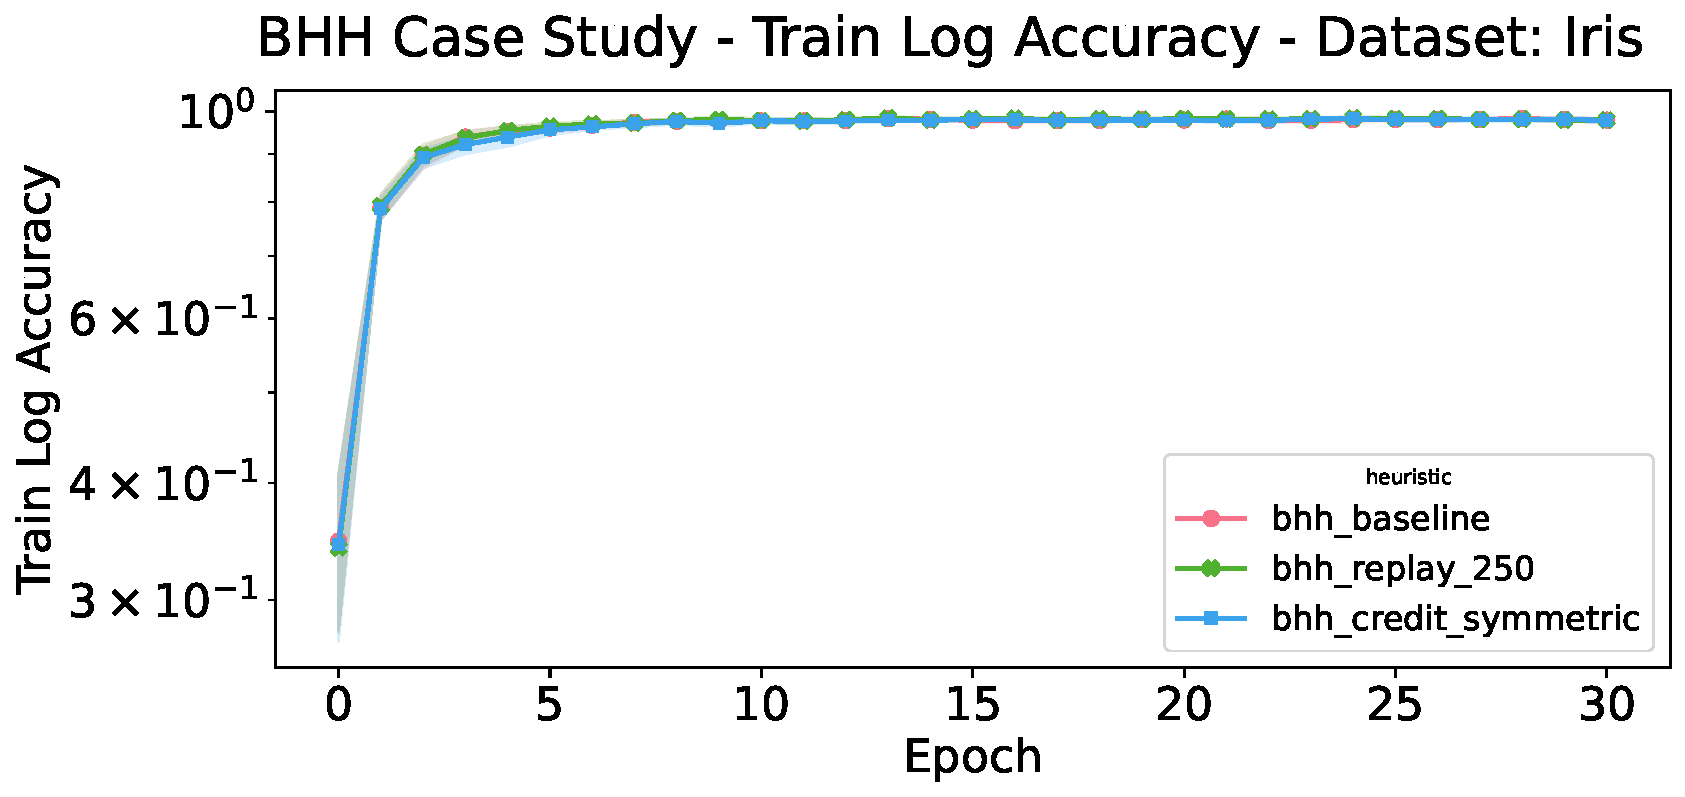
\includegraphics[width=1.0\textwidth]{case_study/metrics/figures/train/train_accuracy.pdf}
		\caption{Train log accuracy}
		\label{fig:results:case_study:metrics:train_accuracy}
	\end{subfigure}
	\begin{subfigure}{0.5\textwidth}
		\centering
		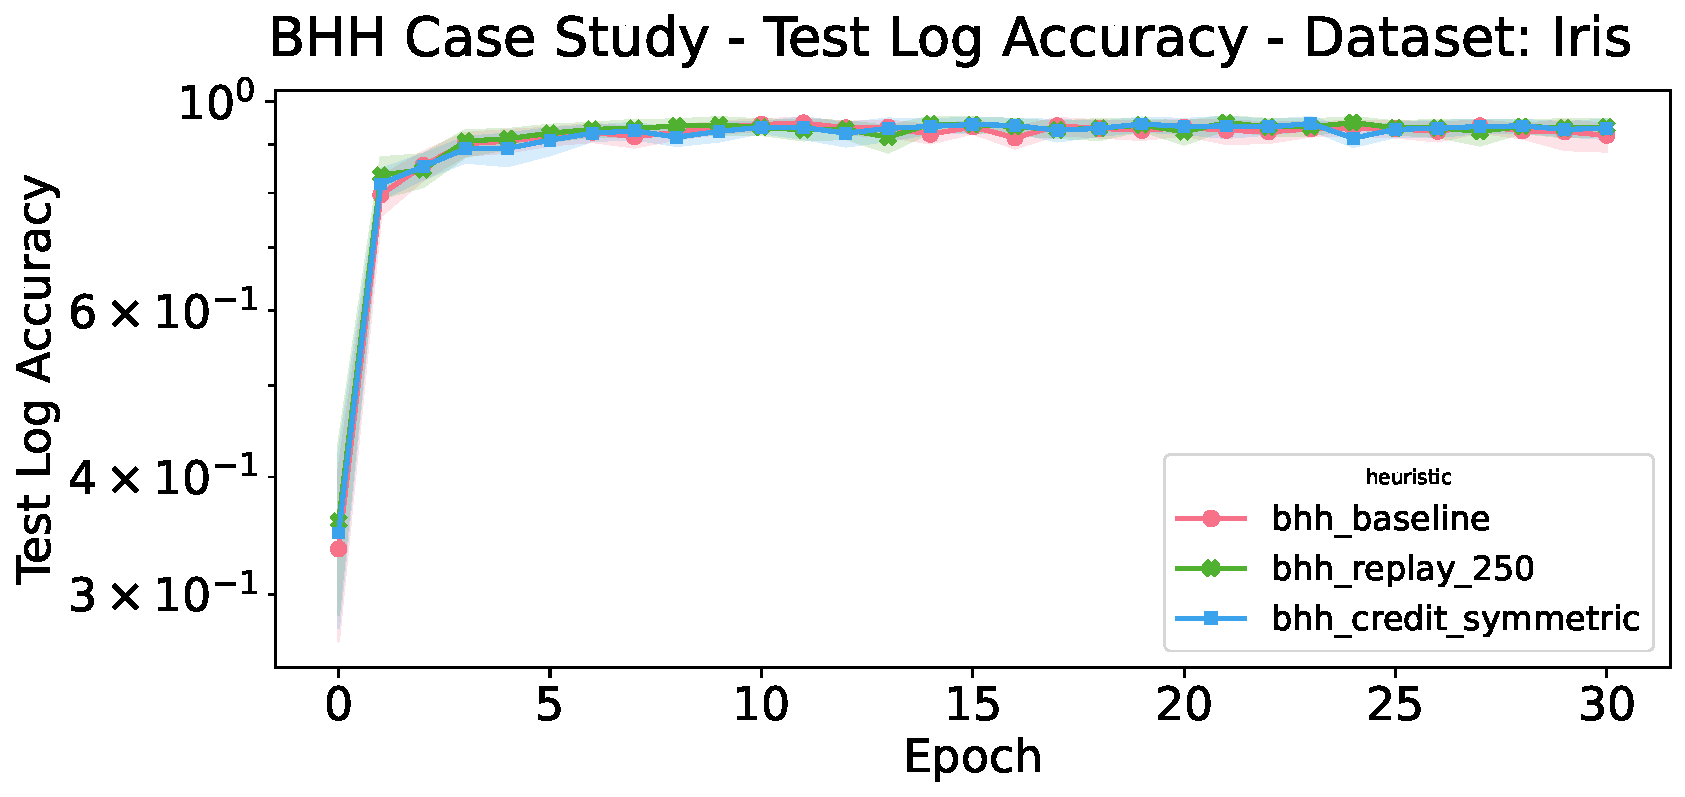
\includegraphics[width=1.0\textwidth]{case_study/metrics/figures/test/test_accuracy.pdf}
		\caption{Test log accuracy}
		\label{fig:results:case_study:metrics:test_accuracy}
	\end{subfigure}
	\par\bigskip
	\caption{The average train and test loss and accuracy plots over 30 epochs, obtained from 30 runs of the case study on the behaviour of the \acs{BHH} on the iris dataset, illustrated in log scale.}
	\label{fig:results:case_study:metrics}
\end{figure}

The first logical observation that can be made is that the \acs{BHH} was indeed able to successfully train the underlying \acs{FFNN}, observed by the convergence of the training process, yielding good results. Figures \ref{fig:results:case_study:metrics:train_accuracy} and \ref{fig:results:case_study:metrics:test_accuracy} show that the trained \acs{FFNN} achieved an accuracy of almost 100\%.



\begin{figure}[htb]
	\begin{subfigure}{0.5\textwidth}
		\centering
		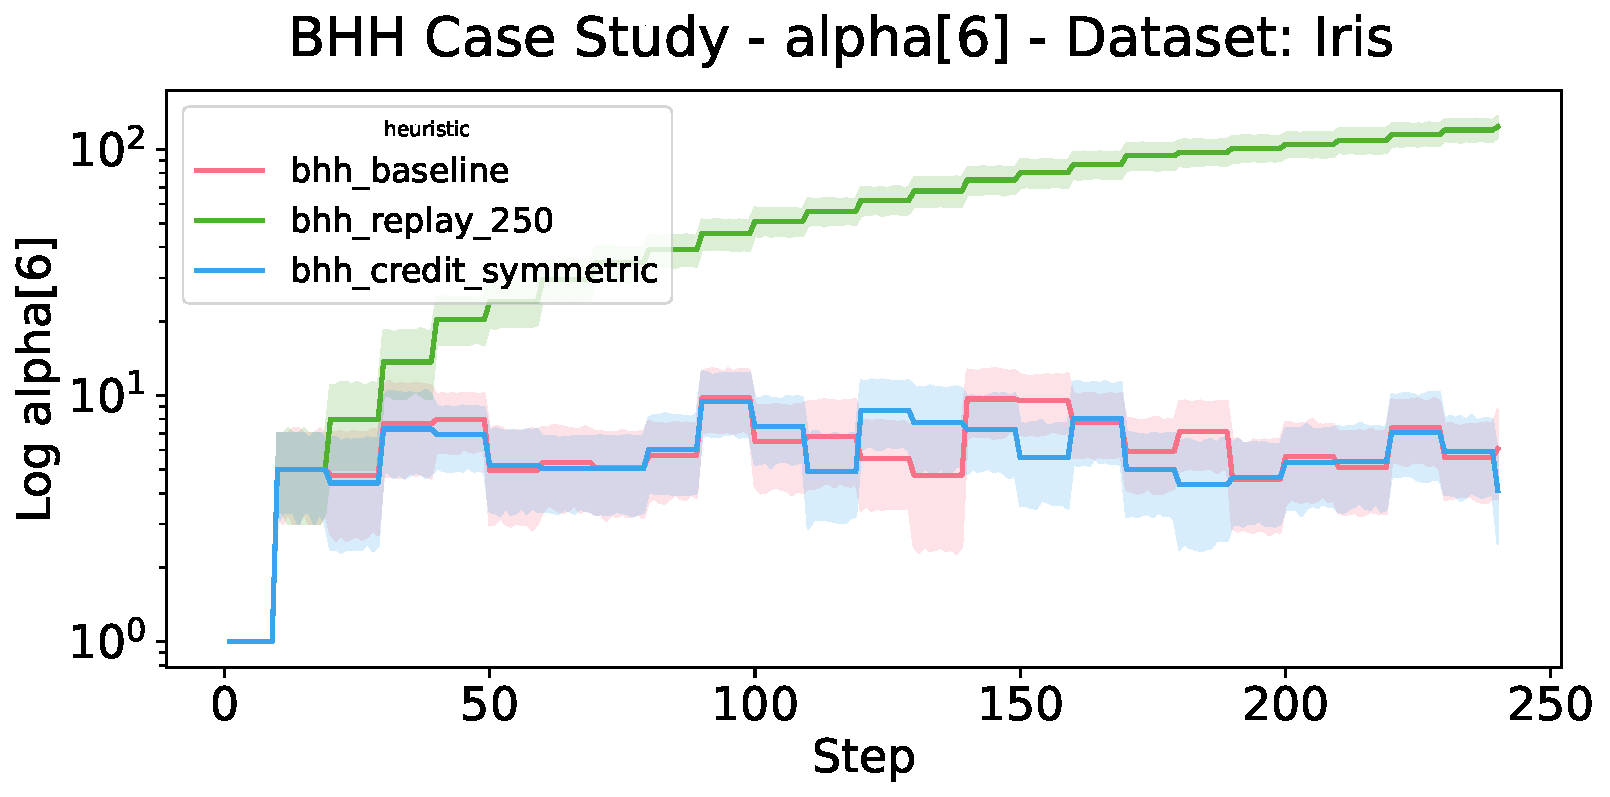
\includegraphics[width=1.0\textwidth]{case_study/params/figures/alphas/alpha[6].pdf}
		\caption{$\alpha_{6}$ - \acs{Adam}}
		\label{fig:results:case_study:alphas:6}
	\end{subfigure}
	\begin{subfigure}{0.5\textwidth}
		\centering
		\includegraphics[width=1.0\textwidth]{case_study/params/figures/thetas/theta[6].pdf}
		\caption{P($\theta_{6} \vert \alpha_{6})$ - \acs{Adam}}
		\label{fig:results:case_study:thetas:6}
	\end{subfigure}
	\par\bigskip
	\begin{subfigure}{0.5\textwidth}
		\centering
		\includegraphics[width=1.0\textwidth]{case_study/params/figures/p_H/p_H[6].pdf}
		\caption{P($h_{6} \vert \theta_{6})$ - \acs{Adam}}
		\label{fig:results:case_study:p_H:6}
	\end{subfigure}
	\begin{subfigure}{0.5\textwidth}
		\centering
		\includegraphics[width=1.0\textwidth]{case_study/params/figures/p_HgEC/p_HgEC[0][6].pdf}
		\caption{$P(h_{6} \vert e_{0}, c_{1})$ - \acs{Adam}}
		\label{fig:results:case_study:p_HgEC:0:6}
	\end{subfigure}
	\par\bigskip
	\caption{The average value of the concentration parameter $\boldsymbol{\alpha}$, at indices 0, 6, 7, and 8 over 240 steps, obtained from 30 runs of the case study on the behaviour of the \acs{BHH} on the iris dataset, illustrated in log scale.}
	\label{fig:results:case_study}
\end{figure}


To illustrate the learning process undergone by the \acs{BHH}, further investigation is required. Consider the concentration parameter $\boldsymbol{\alpha}$ that parameterises the Dirichlet probability distribution, denoted $P(\boldsymbol{\theta} \vert \boldsymbol{\alpha})$. The probability distribution, $P(\boldsymbol{\theta} \vert \boldsymbol{\alpha})$, is used to sample prior \textit{heuristic selection probabilities}. Figures \ref{fig:results:case_study:alphas:0} to \ref{fig:results:case_study:alphas:8} provide illustrations that show that change in values of the concentration parameter $\boldsymbol{\alpha}$, at indices 0, 6, 7, and 8 respectively. Indices 0, 6, 7, and 8 represent the concentration parameters for the \acs{SGD}, \acs{Adam}, \acs{PSO} and \acs{GA} low-level heuristics respectively, and only represent a subset of the elements in $\boldsymbol{\alpha}$ and thus, the heuristic pool. Similar illustrations for the other elements in $\boldsymbol{\alpha}$ are left out for brevity as they contain similar illustrations.

The first logical observation to be made from Figures \ref{fig:results:case_study:alphas:0} to \ref{fig:results:case_study:alphas:8} is the step-wise, increasing nature of $\boldsymbol{\alpha}$ for the bhh\_replay\_250 configuration, illustrated in \textcolor{green}{green}. Since the replay window size is sufficiently large to contain the performance log for all the steps executed in the training process, the \acs{BHH} does not forget past performances of low-level heuristics at all. The value for $\boldsymbol{\alpha}$ is never reset to its initial value of 1.0, and thus, $\boldsymbol{\alpha}$ continues to increase throughout the training process. However, it should be noted that the rate and degree of change is different for different indices of $\boldsymbol{\alpha}$.

The next observations that can be made are for the bhh\_baseline configuration, illustrated in \textcolor{red}{red}, and the bhh\_credit\_symmetric configuration in \textcolor{blue}{blue}. Both these configurations see $\boldsymbol{\alpha}$ being reset to its initial value of 1.0 as regular intervals. This interval is defined by the \textit{reanalysis interval} hyper-parameter. The reanalysis interval dictates the frequency at which Bayesian analysis is conducted on the performance log, maintained by the \acs{BHH}. Bayesian analysis is used to update $\boldsymbol{\alpha}$ only at the reanalysis interval. As a result, small plateaus appear where $\boldsymbol{\alpha}$ does not change.

Furthermore, it is important to mention that a change in $\boldsymbol{\alpha}$ between reanalysis windows does not yet necessarily indicate that the \acs{BHH} is learning. The concentration parameter $\boldsymbol{\alpha}$ tracks the \textit{occurrence} of the random event of observing heuristics (denoted $\boldsymbol{{H}}$). Heuristics can be observed as a result of good performance, by which the \acs{BHH} then learns to frequently reselect these heuristics again, or just by chance through the stochastic nature of probabilistic sampling as implemented by the \acs{BHH}. Further investigation is required to illustrate the learning mechanism of the \acs{BHH}.


The probability distribution of heuristic selection probabilities is denoted by $P(\boldsymbol{\theta} \vert \boldsymbol{\alpha})$, where $\boldsymbol{\theta} \sim Dir(\boldsymbol{\alpha, K})$ are the sampled heuristic selection probabilities.

Figures \ref{fig:results:case_study:thetas:0} to \ref{fig:results:case_study:thetas:8} provide illustrations of the distribution of heuristic selection probabilities, $\boldsymbol{\theta}$, sampled from the probability distribution $P(\boldsymbol{\theta} \vert \boldsymbol{\alpha})$ throughout the training process, and averaged over all 30 runs. These illustrations are presented in log scale. Indices 0, 6, 7, and 8 represent the distribution of heuristic selection probabilities for the \acs{SGD}, \acs{Adam}, \acs{PSO} and \acs{GA} low-level heuristics respectively, and only represent a subset of the distribution of heuristic selection probabilities in $\boldsymbol{\theta}$. Similar illustrations for the other elements in $\boldsymbol{\theta}$ are left out for brevity as they contain similar illustrations.

From the illustrations presented in Figures \ref{fig:results:case_study:thetas:0} to \ref{fig:results:case_study:thetas:8}, a clearer picture of the learning process of the \acs{BHH} is formed. The first important observation to make is for the bhh\_replay\_250 configuration, presented in \textcolor{green}{green}. As a reminder, ten low-level heuristics are included in the heuristic pool, yielding an expected mean heuristics selection probability of 0.1, for each heuristic, by the frequentist view of probabilistic modelling.

Towards the end of the training process, the heuristic selection probability converges back to the symmetrical, uniform probability distribution, yielding a heuristic selection probability of 0.1, for all heuristics. This can be explained as follows: most of the training progress is made in the early stages of the training process, and training converges towards the end of the training process. Since training converges, all heuristics, no matter their past performances, fail to yield better solutions towards the end of the training process. As a result of training convergence, heuristics then fail to meet the performance criteria and credit allocations by means of the credit assignment strategy.

Both the bhh\_baseline (\textcolor{red}{red}) and the bhh\_replay\_250 (\textcolor{green}{green}) configurations make use of the \textit{ibest} credit assignment strategy. The \textit{ibest} credit assignment strategy allocates credit to the heuristic that yields the best performance for the current iteration/step and thus, towards the end of the training process, any random heuristic can yield the best iteration performance. However, since the bhh\_baseline is configured with a small replay window size of 10, and a reanalysis interval of 10, the concentration parameter $\boldsymbol{\alpha}$ is reset to its default value of 1.0 more often than the bhh\_replay\_250 configuration, resulting in a probability distribution that is broader, and thus, explaining the larger variance of $\boldsymbol{\theta}$ throughout.

It should be noted that, despite using the same random seed across configurations for the same run number, the behavioural changes between the configurations start to show after about 30 steps. As a reminder, the bhh\_credit\_symmetric (\textcolor{blue}{blue}) configuration, does not bias towards best performing heuristics. Where the bhh\_baseline and bhh\_replay\_250 configurations then diverge from the behaviour of the bhh\_credit\_symmetric configuration is proof of the effect of performance bias.

Furthermore, it can be observed for small windows, at various steps for multiple runs, that the variance of $\boldsymbol{\theta}$, for the bhh\_baseline configuration and the bhh\_credit\_symmetric configuration, do not yield means that are equal to the expected heuristic selection probabilities of 0.1. This is proof that the \acs{BHH} does not just implement a form of random search, despite having small reanalysis interval and replay window size configurations. This is also true for the bhh\_credit\_symmetric configuration, as the bhh\_credit\_symmetric configuration biases towards heuristics that happen to be sampled, despite not biasing towards good performance.

Finally, the bhh\_baseline configuration and the bhh\_credit\_symmetric configuration both yield similar volatile behaviour, much more so than with the bhh\_replay\_250 configuration. This can be attributed to a very small reanalysis window combined with a small replay window size of 10, that contains very few samples to learn from. A small reanalysis interval and a small replay window size allows for more exploration of the heuristic space, but can also yield greater variance of the heuristic selection probabilities. Once again, any differences then in the behaviour of the bhh\_baseline compared to the bhh\_credit\_symmetric configurations is proof of small performance exploitations and biases by the bhh\_baseline configuration.

The prior heuristic selection probability distribution is denoted $P(\boldsymbol{H} \vert \boldsymbol{\theta})$. As such, $P(\boldsymbol{H} \vert \boldsymbol{\theta}) = \boldsymbol{\theta}$ and heuristics are initially sampled such that $\boldsymbol{H} \sim Cat(\boldsymbol{\theta})$.

Figures \ref{fig:results:case_study:p_H:0} to \ref{fig:results:case_study:p_H:8} provide illustrations of the prior heuristic selection probabilities, denoted by $P(\boldsymbol{H} \vert \boldsymbol{\theta})$, at indices 0, 6, 7, and 8, throughout the training process, and averaged over all 30 runs. Similar to before, these illustrations are also presented in log scale.

The main observation to make from these figures is that they are much less volatile and noisy than the figures presented for the distribution of heuristic selection probabilities, $\boldsymbol{\theta}$, presented in the previous section in Figure \ref{fig:results:case_study:thetas}. This is because of the \textit{reselection} interval hyper-parameter. The reselection interval hyper-parameter is implemented as a way to control the frequency by which new heuristics are selected and allocated to each entity. Since the default \textit{reselection} interval is set to 10, the heuristic selection probabilities are only resampled at intervals of 10. These illustrations then simply yield rough approximations of the illustrations provided in Figures \ref{fig:results:case_study:thetas:0} to \ref{fig:results:case_study:thetas:8} for the distribution of heuristic selection probabilities. As such, the same observations and conclusions that are made in Section \ref{sec:results:case_study:probs_of_select_probs} also apply in this section.

Finally, it should be mentioned that at each step, the goal of the \acs{BHH} is to update these prior ``beliefs'' based on newly observed evidence of heuristic performances. Since these prior heuristic selection probabilities change over time, it can be concluded that the change in prior heuristic selection probabilities is a result of the learning mechanism of the \acs{BHH}. Furthermore, the prior heuristic selection probability distribution provides an opportunity to utilise prior knowledge by some expert before training starts, by injecting heuristic selection biases, by means of the initial values for the concentration parameter $\boldsymbol{\alpha}$.

The posterior heuristic selection probability distribution is defined as $P(\boldsymbol{H} \vert \boldsymbol{E}, \boldsymbol{C}; \boldsymbol{\theta}, \boldsymbol{\phi}, \boldsymbol{\psi})$, where $\boldsymbol{E}$ represents the vector of entities in the entity pool, and $\boldsymbol{C}$ represents the vector of credit allocation outcomes as implemented by the credit assignment strategy. Furthermore $\boldsymbol{\theta}$ and $\boldsymbol{\phi}$ represent the probability distributions of heuristic selection probabilities and the entity selection probabilities respectively. Finally, $\boldsymbol{\psi}$ represents the probability distribution of successful credit allocation probabilities.

Figures \ref{fig:results:case_study:p_HgEC:0:0} to \ref{fig:results:case_study:p_HgEC:0:8} provide illustrations of the calculated posterior heuristic selection probabilities at indices 0, 6, 7, and 8, throughout the training process, averaged over 30 runs. Similar to before, these illustrations are also presented in log scale. As before, illustrations for the other indices are left out for brevity as they yield similar illustrations.

The main observation to make from Figures \ref{fig:results:case_study:p_HgEC:0:0} to \ref{fig:results:case_study:p_HgEC:0:8} is that the implemented posterior heuristic selection distribution, defined by $P(\boldsymbol{H} \vert \boldsymbol{E}, \boldsymbol{C}; \boldsymbol{\theta}, \boldsymbol{\phi}, \boldsymbol{\psi})$, does not yield normalised probabilities, but rather yield unnormalised \textit{logits}, which are used to parameterise a Categorical probability distribution from which new heuristic selections are sampled. The reasons for the aforementioned is because the probabilistic model is evaluated proportionally as was discussed in Section \ref{sec:bhh}. As a reminder, the log-sum-exp trick is used in order to maintain numerical stability, yielding \textit{logits} instead of probabilities.

Another observation to make is for the bhh\_replay\_250 configuration $(\textcolor{green}{green})$. Figures \ref{fig:results:case_study:p_HgEC:0:0} to \ref{fig:results:case_study:p_HgEC:0:8} show that the posterior heuristic selection probabilities converge to the expected heuristic selection probabilities later in the training stages. The aforementioned suggests that the \acs{BHH} is not able to find further performance biases and cannot exploit better solutions. At this point, the \acs{BHH} starts to explore more as the concentration parameters are reanalysed more uniformly, resolving more and more to a random search in attempt to find better solutions.

Furthermore, the posterior heuristic selection probability distribution is conditional on the occurrence of a specific entity that the potential heuristic will be applied to, as well as a specific performance criterion enforced by a specific credit assignment strategy. This means that heuristic selection is specific to each entity. A particular heuristic might be good for one entity, but not for another. This is a strong characteristic of the \acs{BHH}, as it learns to apply the correct heuristic to the correct entity at the correct time in the training process.

Finally, the posterior heuristic selection probabilities are much less volatile than their prior heuristic selection probability equivalents. This is a result of the information that is added in the performance log by tracking the entity and credit allocation as well.

It can be concluded from Sections \ref{sec:results:case_study:performance_metrics} to \ref{sec:results:case_study:posterior_selec_prob} that the \acs{BHH} is able to successfully train the underlying \acs{FFNN} for the case study on the iris dataset. Furthermore it can be concluded that the learning mechanism implemented by the \acs{BHH} is able to exploit minor performance biases, and thus the \acs{BHH} is able to correctly allocate the correct heuristic to the correct entity at the correct time in the training process.

%%%%%%%%%%%%%%%%%%%%%%%%%%%%%%%%%%%%%%%%%%%%%%%%%%%%%%%%%%%%%%%5
% BHH vs. Low-Level Heuristics
%%%%%%%%%%%%%%%%%%%%%%%%%%%%%%%%%%%%%%%%%%%%%%%%%%%%%%%%%%%%%%%5
\subsection{BHH vs. Low-Level Heuristics}\label{sec:results:standalone}

This section provides the empirical results for the experimental group that compares the performance of the \acs{BHH} to the performance of the individual, standalone, low-level heuristics. Detailed discussions and illustrations follow. As a reminder, the set of low-level heuristics includes a number of gradient-based heuristics and a number of \acp{MH}. Three variants of the \acs{BHH} is included in the experiment, including the \acs{BHH} baseline configuration with a heuristic pool that contains all the low-level heuristics (denoted bhh\_all), the \acs{BHH} configuration with a heuristic pool that contains only gradient-based heuristics (denoted bhh\_gd), and finally, the \acs{BHH} configuration with a heuristics pool that contains only \acp{MH} (denoted bhh\_mh).

Table \ref{tab:results:standalone:metrics:loss} presents the empirical results for this experimental group, showing the average test loss and statistics for all the low-level heuristics, compared to the three variants of the \acs{BHH} that was implemented. The test loss is measured at the last epoch for each dataset, over all independent runs.

Table \ref{tab:results:standalone:metrics:loss} shows that the bhh\_gd configuration produced the best results of the \acs{BHH} variants and managed to perform well, producing generally good results across all datasets. The bhh\_gd configuration managed to produce results that are comparable to the top three heuristics for each dataset, while the bhh\_all and bhh\_mh produced average results compared to all the heuristics.

Table \ref{tab:results:standalone:metrics:rank} provides the empirical results from Table \ref{tab:results:standalone:metrics:loss} in ranked format. The performance rank is calculated as the average rank produced by each heuristic, across all datasets, for all independent runs and all epochs. The average rank across all epochs produces a view on the performance of the heuristics as it relates to the entire training process. Finally, a normalised average rank is provided for the overall performance of all heuristics at the bottom of the table. The normalised average rank is calculated as a discrete normalisation of the average rank achieved across all datasets, for all independent runs and epochs.

From the normalised average ranks provided in Table \ref{tab:results:standalone:metrics:rank}, it can be seen that the bhh\_gd configuration ranked fourth, while the bhh\_all and bhh\_mh configurations ranked sixth and eighth amongst all thirteen heuristic implementations respectively. These results show that the \acs{BHH} generally performs well, but is not able to outperform the best heuristic for each dataset.

Figure \ref{fig:results:standalone:descriptive:descriptive} provides an illustration showing a descriptive plot of the average ranks achieved over all independent runs, for each heuristic, per dataset. The heuristics are ordered according to the normalised ranks presented in Table \ref{tab:results:standalone:metrics:rank}.

\begin{figure}[htb]
	\centering
	\includegraphics[width=\textwidth]{standalone/figures/descriptive/descriptive.pdf}
	\caption{Descriptive plots for the average ranks of all low-level heuristics compared to three heuristic pool variants of the \acs{BHH} baseline configuration, per dataset, across all independent runs and epochs.}
	\label{fig:results:standalone:descriptive:descriptive}
\end{figure}

From Figure \ref{fig:results:standalone:descriptive:descriptive} a few observations can be made. Firstly, both \acs{Adam} and \acs{RMSProp} achieved radically different average ranks for the student performance dataset, compared to the other datasets. This can also be seen in Table \ref{tab:results:standalone:metrics:rank}. Further investigation into the reasons for this is required as both these heuristics perform well on all other datasets, and the other heuristics perform well for the student performance dataset. A suggestion is that an invalid learning rate or learning rate schedule leads to a scenario where good solutions are overshot, causing \acs{Adam} and \acs{RMSProp} to struggle to resolve back to good solutions. Furthermore, the bhh\_gd heuristic achieved the lowest variance in average rank across all datasets, compared to the other heuristics. The aforementioned shows the generalisation capabilities of the \acs{BHH} to multiple problems.

Figure \ref{fig:results:standalone:descriptive:cd} provides an illustration of the overall critical difference plots that illustrate the statistically significant differences in ranked performance for each heuristic as it relates to all datasets, across all independent runs and epochs.

\begin{figure}[htb]
	\centering
	\includegraphics[width=\textwidth]{standalone/figures/cd/overall.pdf}
	\caption{Critical difference plots for the average ranks of all low-level heuristics compared to three heuristic pool variants of the baseline \acs{BHH}, across all datasets, runs and epochs.}
	\label{fig:results:standalone:descriptive:cd}
\end{figure}

Although the outcomes of the bhh\_all and bhh\_mh configurations seem to produce average performance results, it should be noted that the performance difference between all heuristics is very small. Furthermore, the best configuration of the \acs{BHH}, namely the bhh\_gd configuration, is statistically only outperformed overall by \acs{Adagrad} and \acs{Adam}, yielding statistically comparable results to \acs{RMSProp} and \acs{NAG}. It should be noted that the standalone low-level heuristics already produce good results in general across all datasets. In this particular case, producing better performance outcomes can be hard to achieve. However, as mentioned previously, the \acs{BHH} provides a generalisation capability across all datasets that is advantageous to the \acs{BHH}.

Another observation that can be made is that the gradient-based heuristics generally performed much better than the \acp{MH} on all datasets. State of the art methods for training \acp{FFNN}, such as \acs{Adam}, utilise gradient-based approaches that have been proven to work well on many occasions \cite{ref:kingma:2014}. Exploration of the heuristic space leads the \acs{BHH} to consider other heuristics during the training process, which could possibly result in worse performances at times. As previously mentioned, a suggestion to improve on these results is to include a move-acceptance strategy, where heuristic progressions are discarded if they fail to produce better results.